%%% template.tex
%%%
%%% This LaTeX source document can be used as the basis for your technical
%%% paper or abstract.
%%%
%%% This example is tailored toward the two-page abstract. Please see "template.tex"
%%% for a more fully-annotated example.

\documentclass{acmsiggraph}

%%% Title of your article or abstract.

\title{GPGPU View-frustum Culling for Particle systems}

\author{Henrik Johansson}
\pdfauthor{Henrik Johansson}

%%% Used by the ``review'' variation; the online ID will be printed on 
%%% every page of the content.

\TOGonlineid{45678}

% User-generated keywords.

\keywords{GPGPU, Compute, Indirect Draw, Particles, View-frustum}

% With the "\setcopyright" command the appropriate rights management text will be added
% to your document.

%\setcopyright{none}
%\setcopyright{acmcopyright}
%\setcopyright{acmlicensed}
\setcopyright{rightsretained}
%\setcopyright{usgov}
%\setcopyright{usgovmixed}
%\setcopyright{cagov}
%\setcopyright{cagovmixed}
%\setcopyright{rightsretained}

% The year of publication in the "\copyrightyear" command.

\copyrightyear{2016}

%%% Conference information, from the completed rights management form.
%%% The "\conferenceinfo" command has two parameters: 
%%%    - conference name
%%%    - conference date and location
%%% The "\isbn" field includes the year and month after the article ISBN.

\conferenceinfo{SIGGRAPH 2016 Posters}{July 24-28, 2016, Anaheim, CA} 
\isbn{978-1-4503-ABCD-E/16/07} 
\doi{http://doi.acm.org/10.1145/9999997.9999999}

\begin{document}

%%% This is the ``teaser'' command, which puts an figure, centered, below 
%%% the title and author information, and above the body of the content.

 \teaser{
   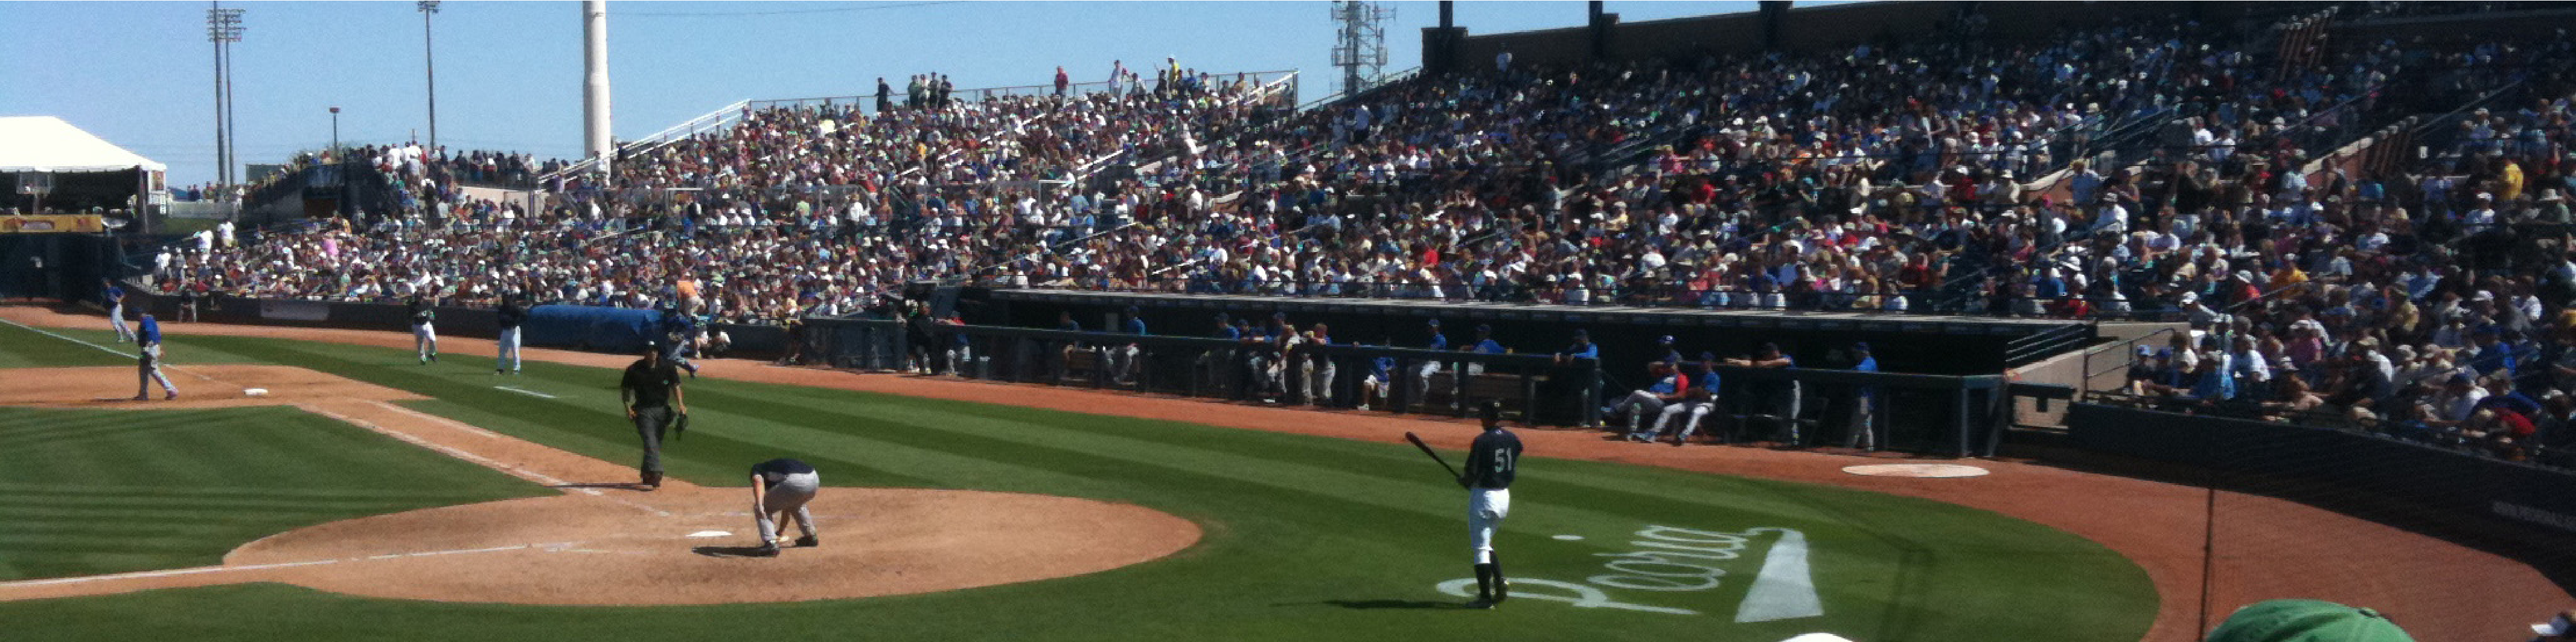
\includegraphics[height=1.5in]{images/sampleteaser}
   \caption{Spring Training 2009, Peoria, AZ.}
 }

\maketitle

\begin{abstract}

(what does this article talk about and what was the result)

\end{abstract}


% The next three commands are required, and insert the user-generated keywords, 
% The CCS concepts list, and the rights management text.
% Please make sure there is a blank line between each of these three commands.

\keywordlist

\section{Introduction}

(How does particle systems work in modern games)

\section{Relevance}

Particle systems are used in almost every game. They are used to model everything from explosions and smoke effect to weather effects such as snow or rain. One big advantage for particle systems is that they do not rely as much on user generated content since most of them are based on mathematical formulas. 

\begin{figure}[ht]
  \centering
  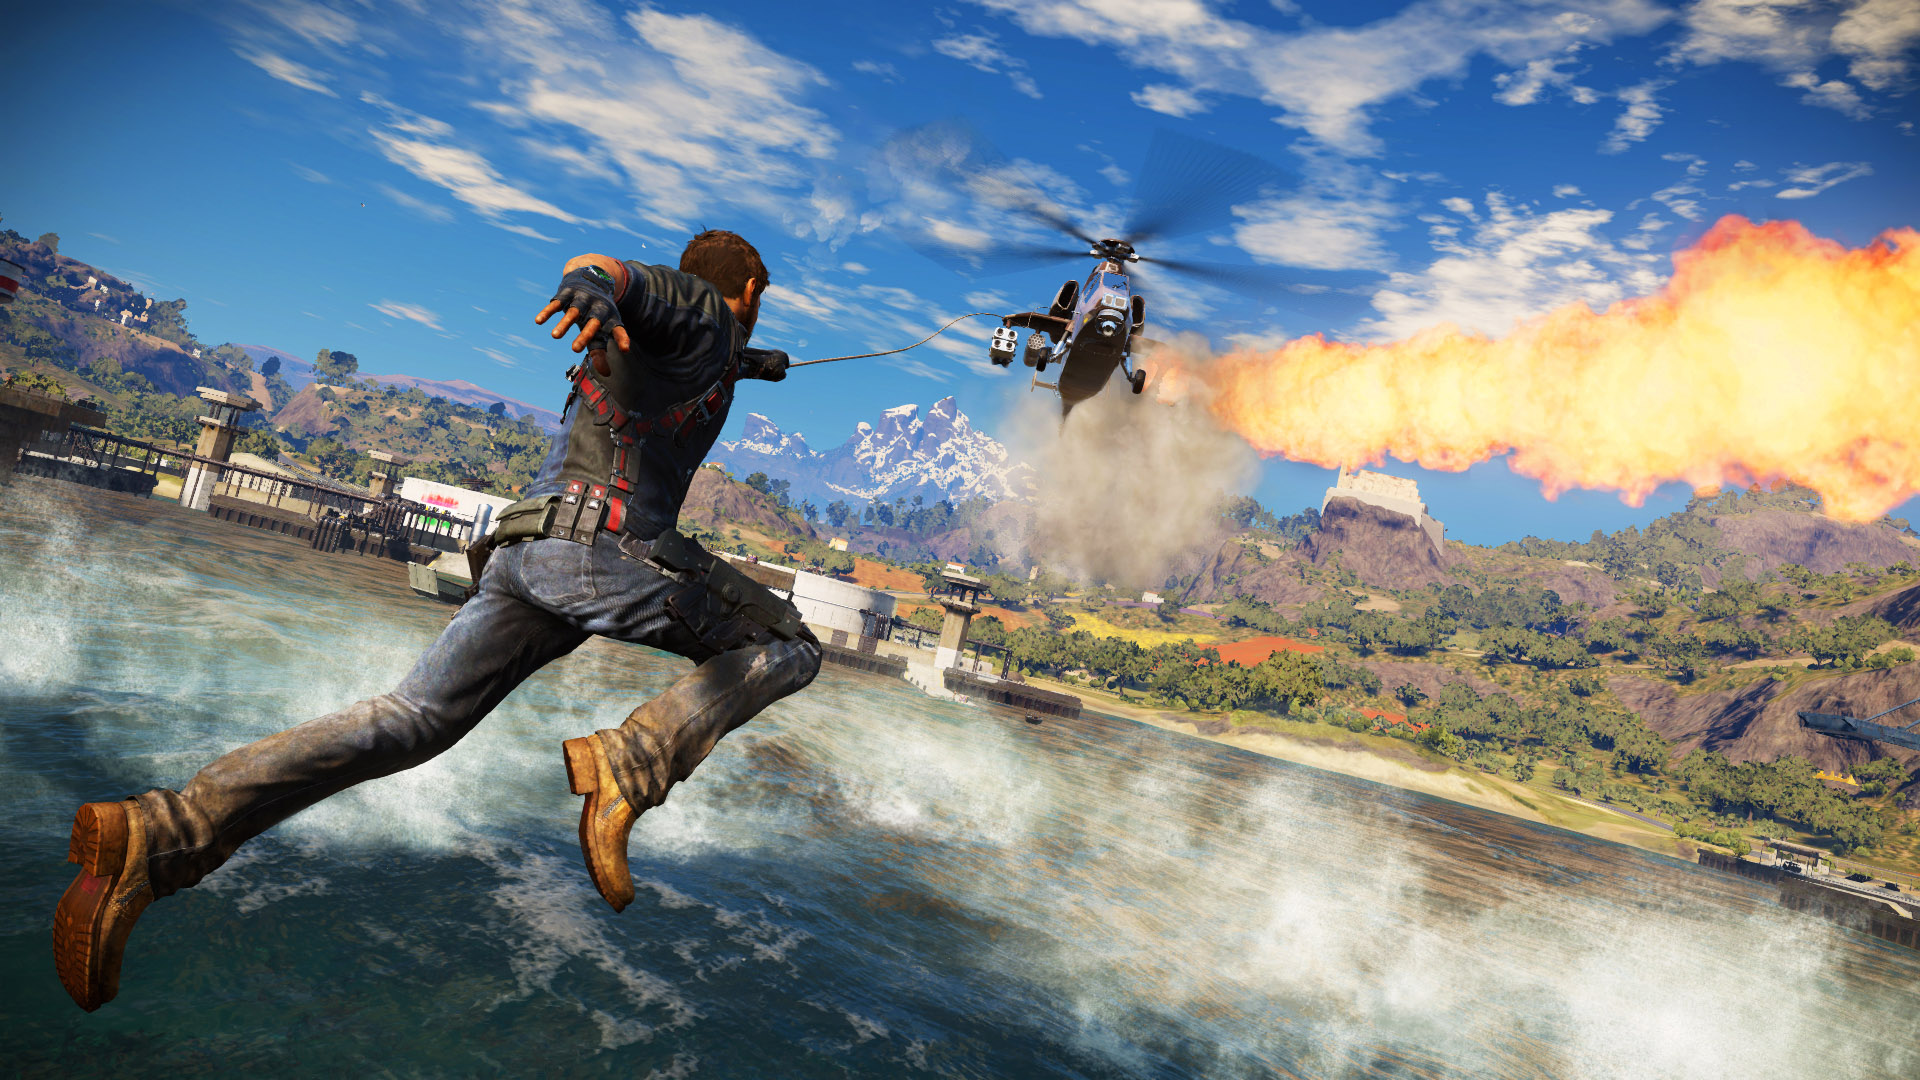
\includegraphics[width=3.0in]{images/jc3.jpg}
  \caption{Just Cause 3, Image from verge.com}
  \label{fig:ferrari}
\end{figure}

\section{Problem}
(What drawbacks does the current way of doing it have)

\section{Solution}
(explain the solution)

\section{Result}
(explain the test)
(show graphs and some data)

\section{Discussion}
(discuss the data and why it is relevant)
(discuss future work)

\section{Conclusion}
(talk about the end results )

\bibliographystyle{acmsiggraph}
\nocite{*}
\bibliography{template}
\end{document}
